\documentclass[11pt]{article}
\usepackage{url}
\usepackage{listings}
\usepackage{tikz}
%\usepackage{algorithm2e}
\usetikzlibrary{arrows,automata,shapes}
\tikzstyle{block} = [rectangle, draw, fill=blue!20, 
    text width=5em, text centered, rounded corners, minimum height=2em]
\tikzstyle{bt} = [rectangle, draw, fill=blue!20, 
    text width=1em, text centered, rounded corners, minimum height=2em]

\lstset{ %
language=Java,
basicstyle=\ttfamily,commentstyle=\scriptsize\itshape,showstringspaces=false,breaklines=true,numbers=left}

\newtheorem{defn}{Definition}
\newtheorem{crit}{Criterion}
\newcommand{\true}{\mbox{\sf true}}
\newcommand{\false}{\mbox{\sf false}}

\newcommand{\handout}[5]{
  \noindent
  \begin{center}
  \framebox{
    \vbox{
      \hbox to 5.78in { {\bf Software Testing, Quality Assurance and Maintenance } \hfill #2 }
      \vspace{4mm}
      \hbox to 5.78in { {\Large \hfill #5  \hfill} }
      \vspace{2mm}
      \hbox to 5.78in { {\em #3 \hfill #4} }
    }
  }
  \end{center}
  \vspace*{4mm}
}

\newcommand{\lecture}[4]{\handout{#1}{#2}{#3}{#4}{Lecture #1}}
\topmargin 0pt
\advance \topmargin by -\headheight
\advance \topmargin by -\headsep
\textheight 8.9in
\oddsidemargin 0pt
\evensidemargin \oddsidemargin
\marginparwidth 0.5in
\textwidth 6.5in

\parindent 0in
\parskip 1.5ex
%\renewcommand{\baselinestretch}{1.25}
\lstdefinelanguage{JavaScript}{
  keywords={typeof, new, true, false, catch, function, return, null, catch, switch, var, if, in, while, do, else, case, break},
  keywordstyle=\color{blue}\bfseries,
  ndkeywords={class, export, boolean, throw, implements, import, this},
  ndkeywordstyle=\color{darkgray}\bfseries,
  identifierstyle=\color{black},
  sensitive=false,
  comment=[l]{//},
  morecomment=[s]{/*}{*/},
  commentstyle=\color{purple}\ttfamily,
  stringstyle=\color{red}\ttfamily,
  morestring=[b]',
  morestring=[b]''
}

\usepackage{fontspec}
\setmonofont{Cousine}[Scale=MatchLowercase]

\begin{document}

\lecture{13 --- February 1, 2017}{Winter 2017}{Patrick Lam}{version 0}

We'll wrap up our unit on defining test suites by exploring the question
``How much is enough?'' We'll discuss coverage first and then mutation testing
as ways of answering this question.

First, we can look at actual test suites and see how much coverage they achieve.
I collected this data a few years ago, measured with the EclEmma tool.

\begin{center}
  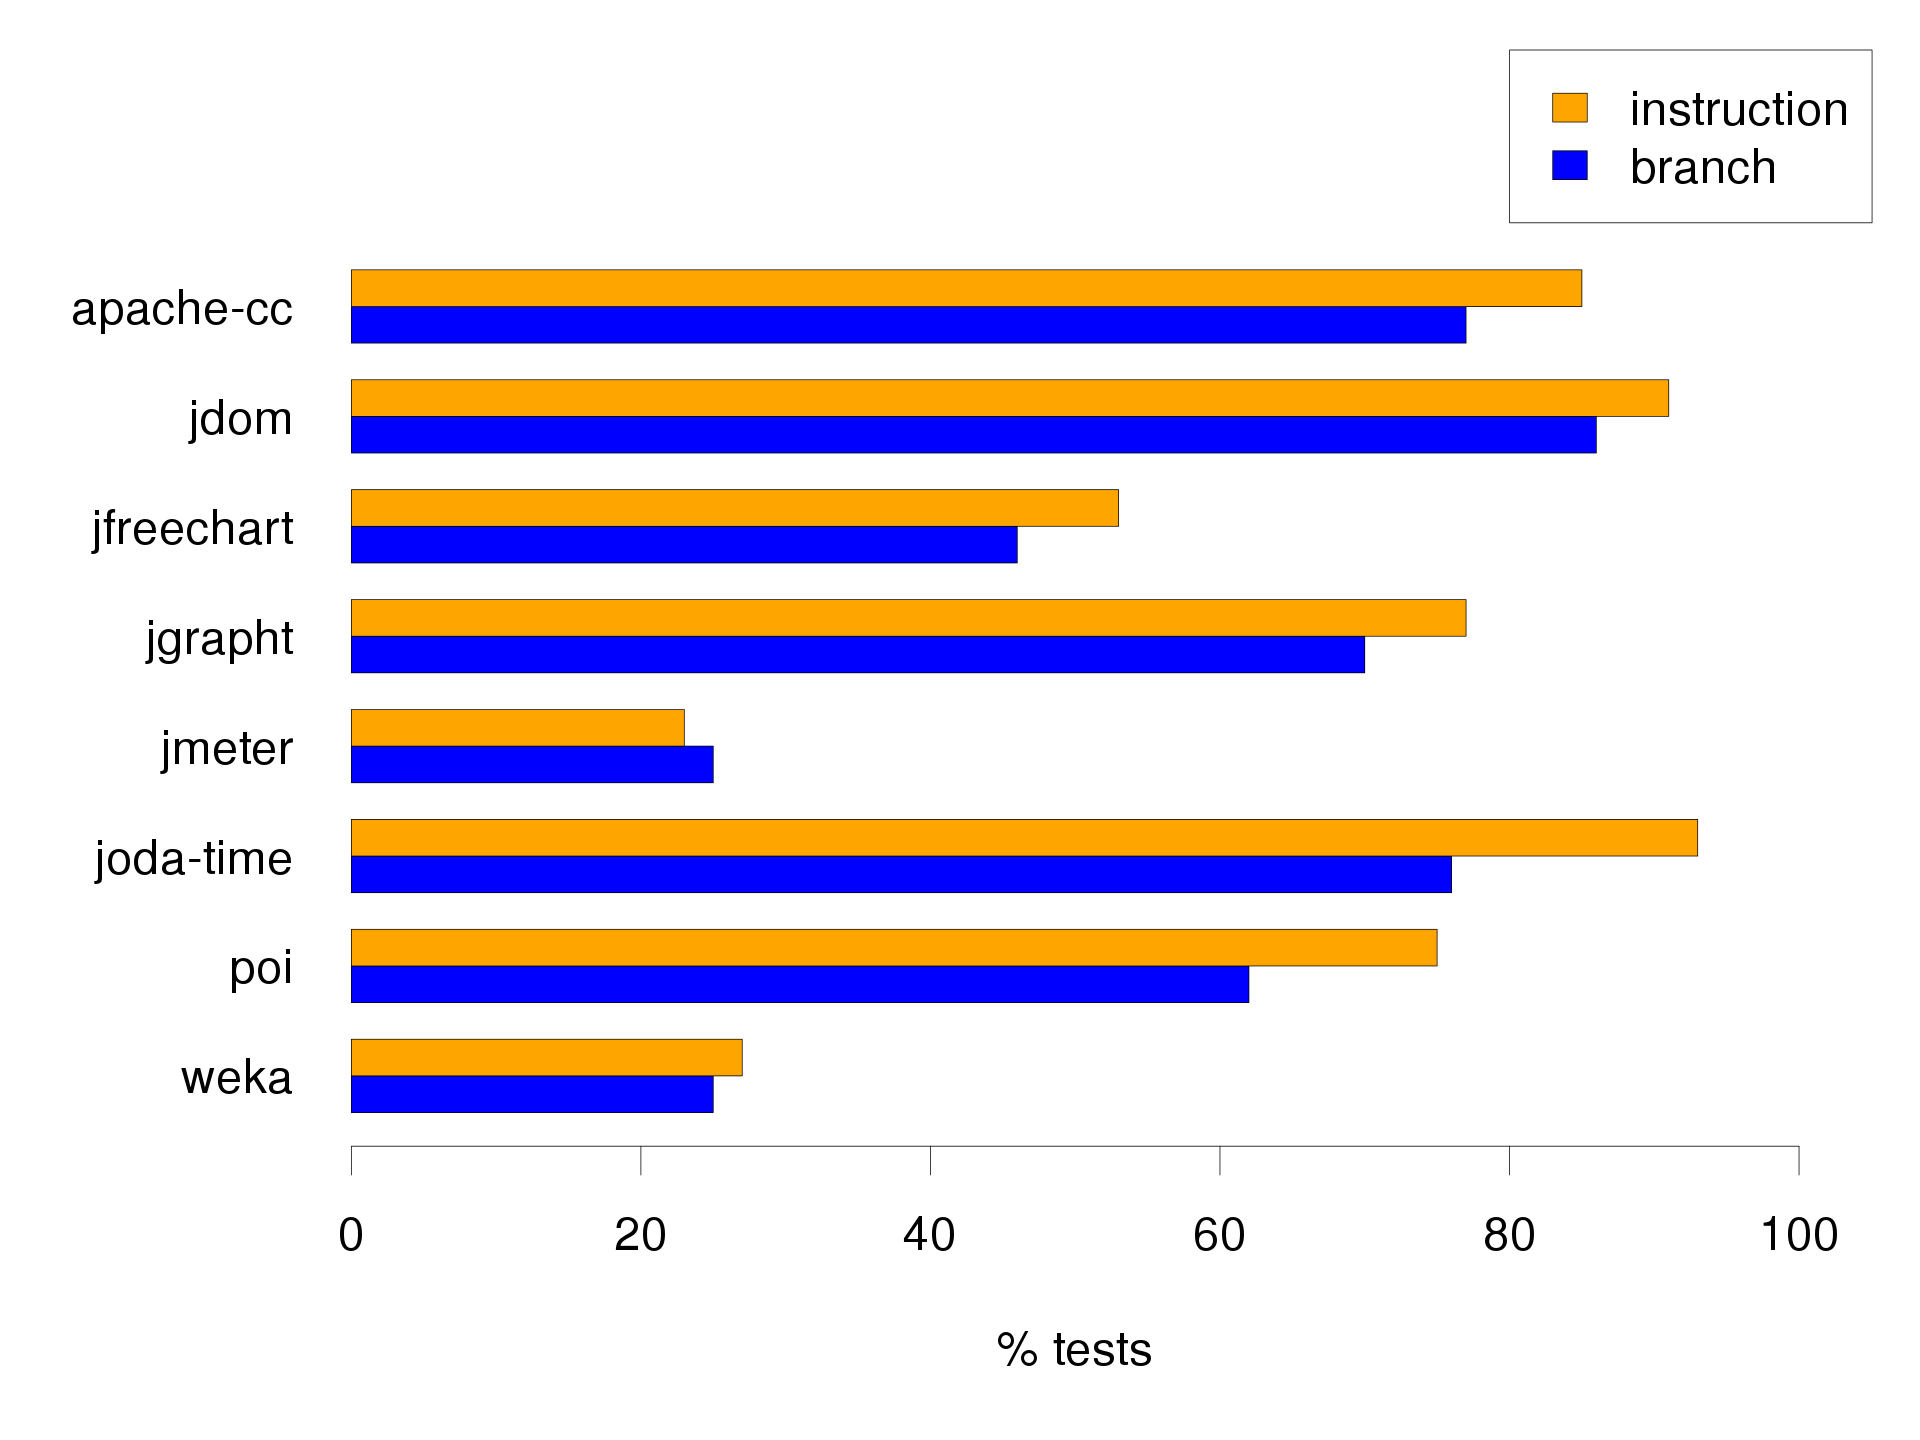
\includegraphics[height=2in]{L13/coverage.png}
\end{center}

We can see that the coverage varies between 20\% and 95\% on actual
open-source projects. I investigated further and found that while Weka has low
test coverage, it instead uses scientific peer review for QA: its features
come from published articles. Common practice in industry is that about 80\%
coverage (doesn't matter which kind) is good enough.

There is essentially no quantitative analysis of input space coverage;
for most purposes, input spaces are essentially infinite.

Let's look at a more specific case study, JUnit. The rest of this lecture is
based on a blog post by Arie van Deursen:

\begin{center}
  \url{https://avandeursen.com/2012/12/21/line-coverage-lessons-from-junit/}
\end{center}

Although you might think of JUnit as something that just magically exists in the world,
it is a software artifact too. JUnit is written by developers who obviously really care
about testing. Let's see what they do.

\newpage

Here's the Cobertura report for JUnit:

\begin{center}
  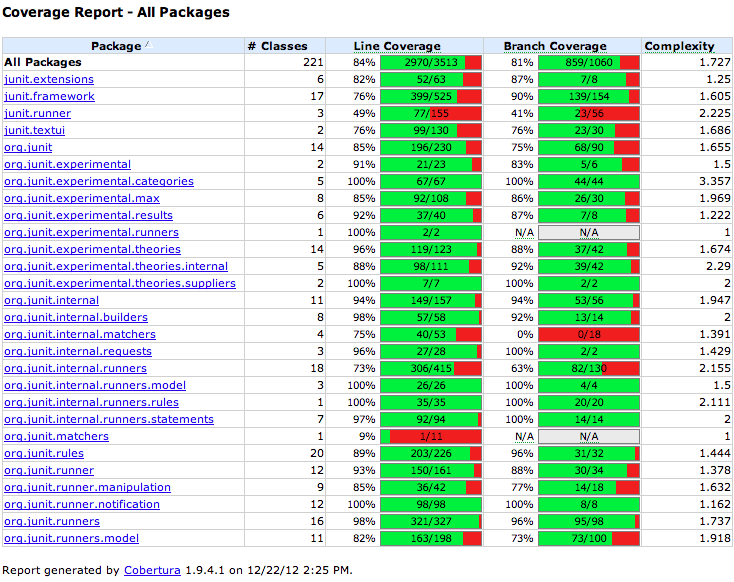
\includegraphics[height=2in]{L13/cobertura-junit.png}
\end{center}

\paragraph{Stats.} Overall instruction (statement) coverage for JUnit 4.11 is about 85\%; there are
13,000 lines of code and 15,000 lines ot test code. (It's not that
unusual for there to be more tests than code.) This is consistent with
the industry average.

\paragraph{Deprecated code?} Sometimes library authors decide that some functionality
was not a good idea after all. In that case they might \emph{deprecate} some methods or
classes, signalling that these APIs will disappear in the future.

In JUnit, deprecated and older code has lower coverage levels. Its 13 deprecated
classes have only 65\% instruction coverage. Ignoring deprecated code, JUnit achieves
93\% instruction coverage. Furthermore, newer code in
package {\tt org.junit.*} has 90\% instruction coverage, while older code in
{\tt junit.*} has 70\% instruction coverage.

(Why is this? Perhaps the coverage decreased over time for the deprecated code, since
no one is really maintaining it anymore, and failing test cases just get removed.)

\paragraph{Untested class.} The blog post points out one class that was completely
untested, which is unusual for JUnit. It turns out that the code came with tests,
but that the tests never got run because they were never added to any test suites.
Furthermore, these tests also failed, perhaps because no one had ever tried them.
The continuous integration infrastructure did not detect this change. (More on CI
later.)

\paragraph{What else?} Arie van Deursen characterizes the remaining 6\% as
``the usual suspects''. In JUnit's case, there was no method with more than
2 to 3 uncovered lines. Here's what he found.

\noindent
\emph{Too simple to test.} Sometimes it doesn't make sense to test a method, because
it's not really doing anything. For instance:
\begin{lstlisting}[language=Java]
  public static void assumeFalse(boolean b) {
    assumeTrue(!b);
  }
\end{lstlisting}
or just getters or {\tt toString()} methods (which can still be wrong).

The empty method is also too simple to test; one might write such a method to allow
it to be overridden in subclasses:
\begin{lstlisting}[language=Java]
  /**
  * Override to set up your specific external resource.
  *
  * @throws if setup fails (which will disable {@code after}
  */
  protected void before() throws Throwable {
    // do nothing
  }
\end{lstlisting}

\noindent \emph{Dead by design.} Sometimes a method really should never be called,
for instance a constructor on a class that should never be instantiated:
\begin{lstlisting}[language=Java]
  /**
  * Protect constructor since it is a static only class
  */
  protected Assert() { }
\end{lstlisting}

A related case is code that should never be executed:
\begin{lstlisting}[language=Java]
  catch (InitializationError e) {
    throw new RuntimeException(
    "Bug in saff's brain: " +
    "Suite constructor, called as above, should always complete");
  }
\end{lstlisting}
Similarly, switch statements may have unreachable default cases. Or other unreachable code.
Sometimes the code is just highly unlikely to happen:
\begin{lstlisting}[language=Java]
  try {
    ...
  } catch (InitializationError e) {
    return new ErrorReportingRunner(null, e); // uncovered
  }
\end{lstlisting}

\paragraph*{Conclusions.} We explored empirically the instruction coverage of JUnit,
which is written by people who really care about testing. Don't forget
that coverage doesn't actually guarantee, by itself, that your code is
well-exercised; what is in the tests matters too. For non-deprecated
code, they achieved 93\% instruction coverage, and so it really is
possible to have no more than 2-3 untested lines of code per
method. It's probably OK to have lower coverage for deprecated
code. Beware when you are adding a class and check that you are also
testing it.

\end{document}

